\section{Auswertung}
\label{sec:Auswertung}

\subsection{Messung des Erdmagnetfeldes und Bestimmung der Resonanzen}
\label{subsec:Erdmagnetfeld}

Bei ausgeschaltetem RF-Feld ist nach aufbauen der Apparatur ein breiter Peak zu sehen, der durch Kompensation der Erdmagnetfelder verkleinert werden sollen.
Das dem Erdmagnetfeld entgegengerichtete Vertikalfeld ist dabei auf den folgenden Wert eingestellt worden,
\begin{align*}
    B_{\text{vertikal}} = \SI{36.013}{\micro\tesla}.
\end{align*}
Es wird die Stärke des gesamten horizontal angelegten Magnetfeldes aus der Abhängigkeit mit der Resonanzfrequenz der beiden Rubidium Isotope $^{87}\text{Rb}$ und $^{85}\text{Rb}$
bestimmt. Dabei wird neben dem Sweep-Magnetfeld noch ein weiteres, horizontales Magnetfeld angelegt. Für das gesamte Magnetfeld folgt dabei,
\begin{align}
    B=B_{\text{sweep}} + B_{\text{horizontal}}.
\end{align}
Da an dem Gerät nur der Strom abzulesen ist, wird das Magnetfeld mithilfe der Gleichung der magnetischen Feldstärke innerhalb eines Helmholtz-Spulenpaares,
\begin{align}
    B=\mu_0\frac{8IN}{\sqrt{125}R}
\end{align}
berechnet. Dabei ist $I$ der abgelesene Strom, $N$ die Windungszahl des Spulenpaares und $R$ der Radius der Spulen.
In \autoref{tab:DatenIsotop1} und \autoref{tab:DatenIsotop2} sind die in dem Versuch gemessenen Daten zur Bestimmung der Resonanz in Abhängigkeit der eingestellten Resonanzfrequenzen
$f_{\text{RF}}$ für das jeweilige Isotop aufgetragen. Mithilfe dieser Daten wurden in \autoref{fig:plot1} und \autoref{fig:plot2} die Daten gegen eine lineare Regression der Form
\begin{align}
    B=a\cdot f_{\text{RF}} + b
\end{align}
ausgewertet. Dabei sind die grün markierten Messwerte aus den Berechnungen ausgeschlossen worden, da sie zu sehr von den anderen Messwerten abwichen.
Es ergeben sich für die beiden Isotope die folgenden Regressionswerte,
\begin{align*}
    a_1 &= \SI{1.4093 \pm 0.015 e-10}{\mega\hertz\per\tesla}, \\
    b_1 &= \SI{2.68 \pm 0.09 e-5}{\tesla}, \\
    a_2 &= \SI{2.066 \pm 0.034 e-10}{\mega\hertz\per\tesla}, \\
    b_2 &= \SI{2.88 \pm 0.21 e-5}{\tesla}.
\end{align*}

\begin{table}[H]
    \centering
    \caption{Messdaten zu den Resonanzpositionen des ersten Isotops.}
    \label{tab:DatenIsotop1}
    \begin{tabular}{c c c}
        \toprule
        $f_{\text{RF}}$ / $\si{\mega\hertz}$ & $I_{\text{sweep}}$ / $\si{\ampere}$  & $I_{\text{horizontal}}$ / $\si{\ampere}$ \\
        \midrule
        0.1  &  0.657  &   0.0    \\
        0.2  &  0.758  &   0.014  \\
        0.3  &  0.275  &   0.059  \\
        0.4  &  0.378  &   0.068  \\
        0.5  &  0.476  &   0.078  \\
        0.6  &  0.164  &   0.115  \\
        0.7  &  0.137  &   0.133  \\
        0.8  &  0.909  &   0.127  \\
        0.9  &  0.203  &  0.191   \\
        1.0  &  0.296  &   0.199  \\
        \bottomrule
    \end{tabular}
\end{table}

\begin{table}[H]
    \centering
    \caption{Messdaten zu den Resonanzpositionen des zweiten Isotops.}
    \label{tab:DatenIsotop2}
    \begin{tabular}{c c c}
        \toprule
        $f_{\text{RF}}$ / $\si{\mega\hertz}$ & $I_{\text{sweep}}$ / $\si{\ampere}$  & $I_{\text{horizontal}}$ / $\si{\ampere}$ \\
        \midrule
        0.1  &  0.776  &  0.0  \\
        0.2  &  0.994  &  0.014  \\
        0.3  &  0.634  &  0.059  \\
        0.4  &  0.852  &  0.068  \\
        0.5  &  0.065  &  0.078  \\
        0.6  &  0.875  &  0.115  \\
        0.7  &  0.966  &  0.133  \\
        0.8  &  0.476  &  0.127  \\
        0.9  &  0.84  &  0.191 \\
        1.0  &  0.932  &  0.199  \\
        \bottomrule
    \end{tabular}
\end{table}

\begin{figure}[H]
    \centering
    \includegraphics[width=0.7\textwidth]{build/Isotop1.pdf}
    \caption{Grafische Auswertung der Messdaten des ersten Isotops.}
    \label{fig:plot1}
\end{figure}

\begin{figure}[H]
    \centering
    \includegraphics[width=0.7\textwidth]{build/Isotop2.pdf}
    \caption{Grafische Auswertung der Messdaten des zweiten Isotops.}
    \label{fig:plot2}
\end{figure}

\subsection{Bestimmung der Landé-Faktoren und der Kernspins}
\label{subsec:lande}

Zur Bestimmung der Landé-Faktoren wird die Gleichung 
\begin{align}
    \omega_0=g_F\frac{\mu_B}{h}B\ \text{mit}\ a=\frac{h}{\mu_B}g_F
\end{align}
nach den Landé-Faktoren $g_F$ umgestellt, wobei $h$ das Plank'sche Wirkungsquantum, $\mu_B$ das Bohr'sche Magneton und $a$ die in \autoref{subsec:Erdmagnetfeld} ausgerechnete Steigung ist.
Es ergeben sich die folgenden Werte,
\begin{align*}
    g_{F_1} &= 0.50710 \pm 0.00552, \\
    g_{F_2} &= 0.34578 \pm 0.00571.
\end{align*}

\noindent
Der Kernspin lässt sich mithilfe der Gleichung (\ref{eq:gf}) berechnen. Mit den Quantenzahlen $J=S=\frac 12$ und $L=0$ für Rubidium \cite{Anleitung21} ergeben sich die folgenden
Kernspins für die jeweiligen Isotope
\begin{align*}
    I_1 &= 1.80066 \pm 0.02505, \\
    I_2 &= 2.87399 \pm 0.05568.
\end{align*}

\subsection{Bestimmung des Isotopenverhältnisses}
\label{subsec:isotopenverhaeltnis}

Zur Bestimmung des Isotopenverhältnisses wird eine Aufnahme des Oszilloskopes bei $f_{\text{RF}} = \SI{100}{\kilo\hertz}$ gemacht und aus dem Verhältnis der Amplituden auf das
Verhältnis der Isotope geschlossen. Die Aufnahme des Oszilloskopes ist in \autoref{fig:Oszilloskop} zu sehen.

\begin{figure}[H]
    \centering
    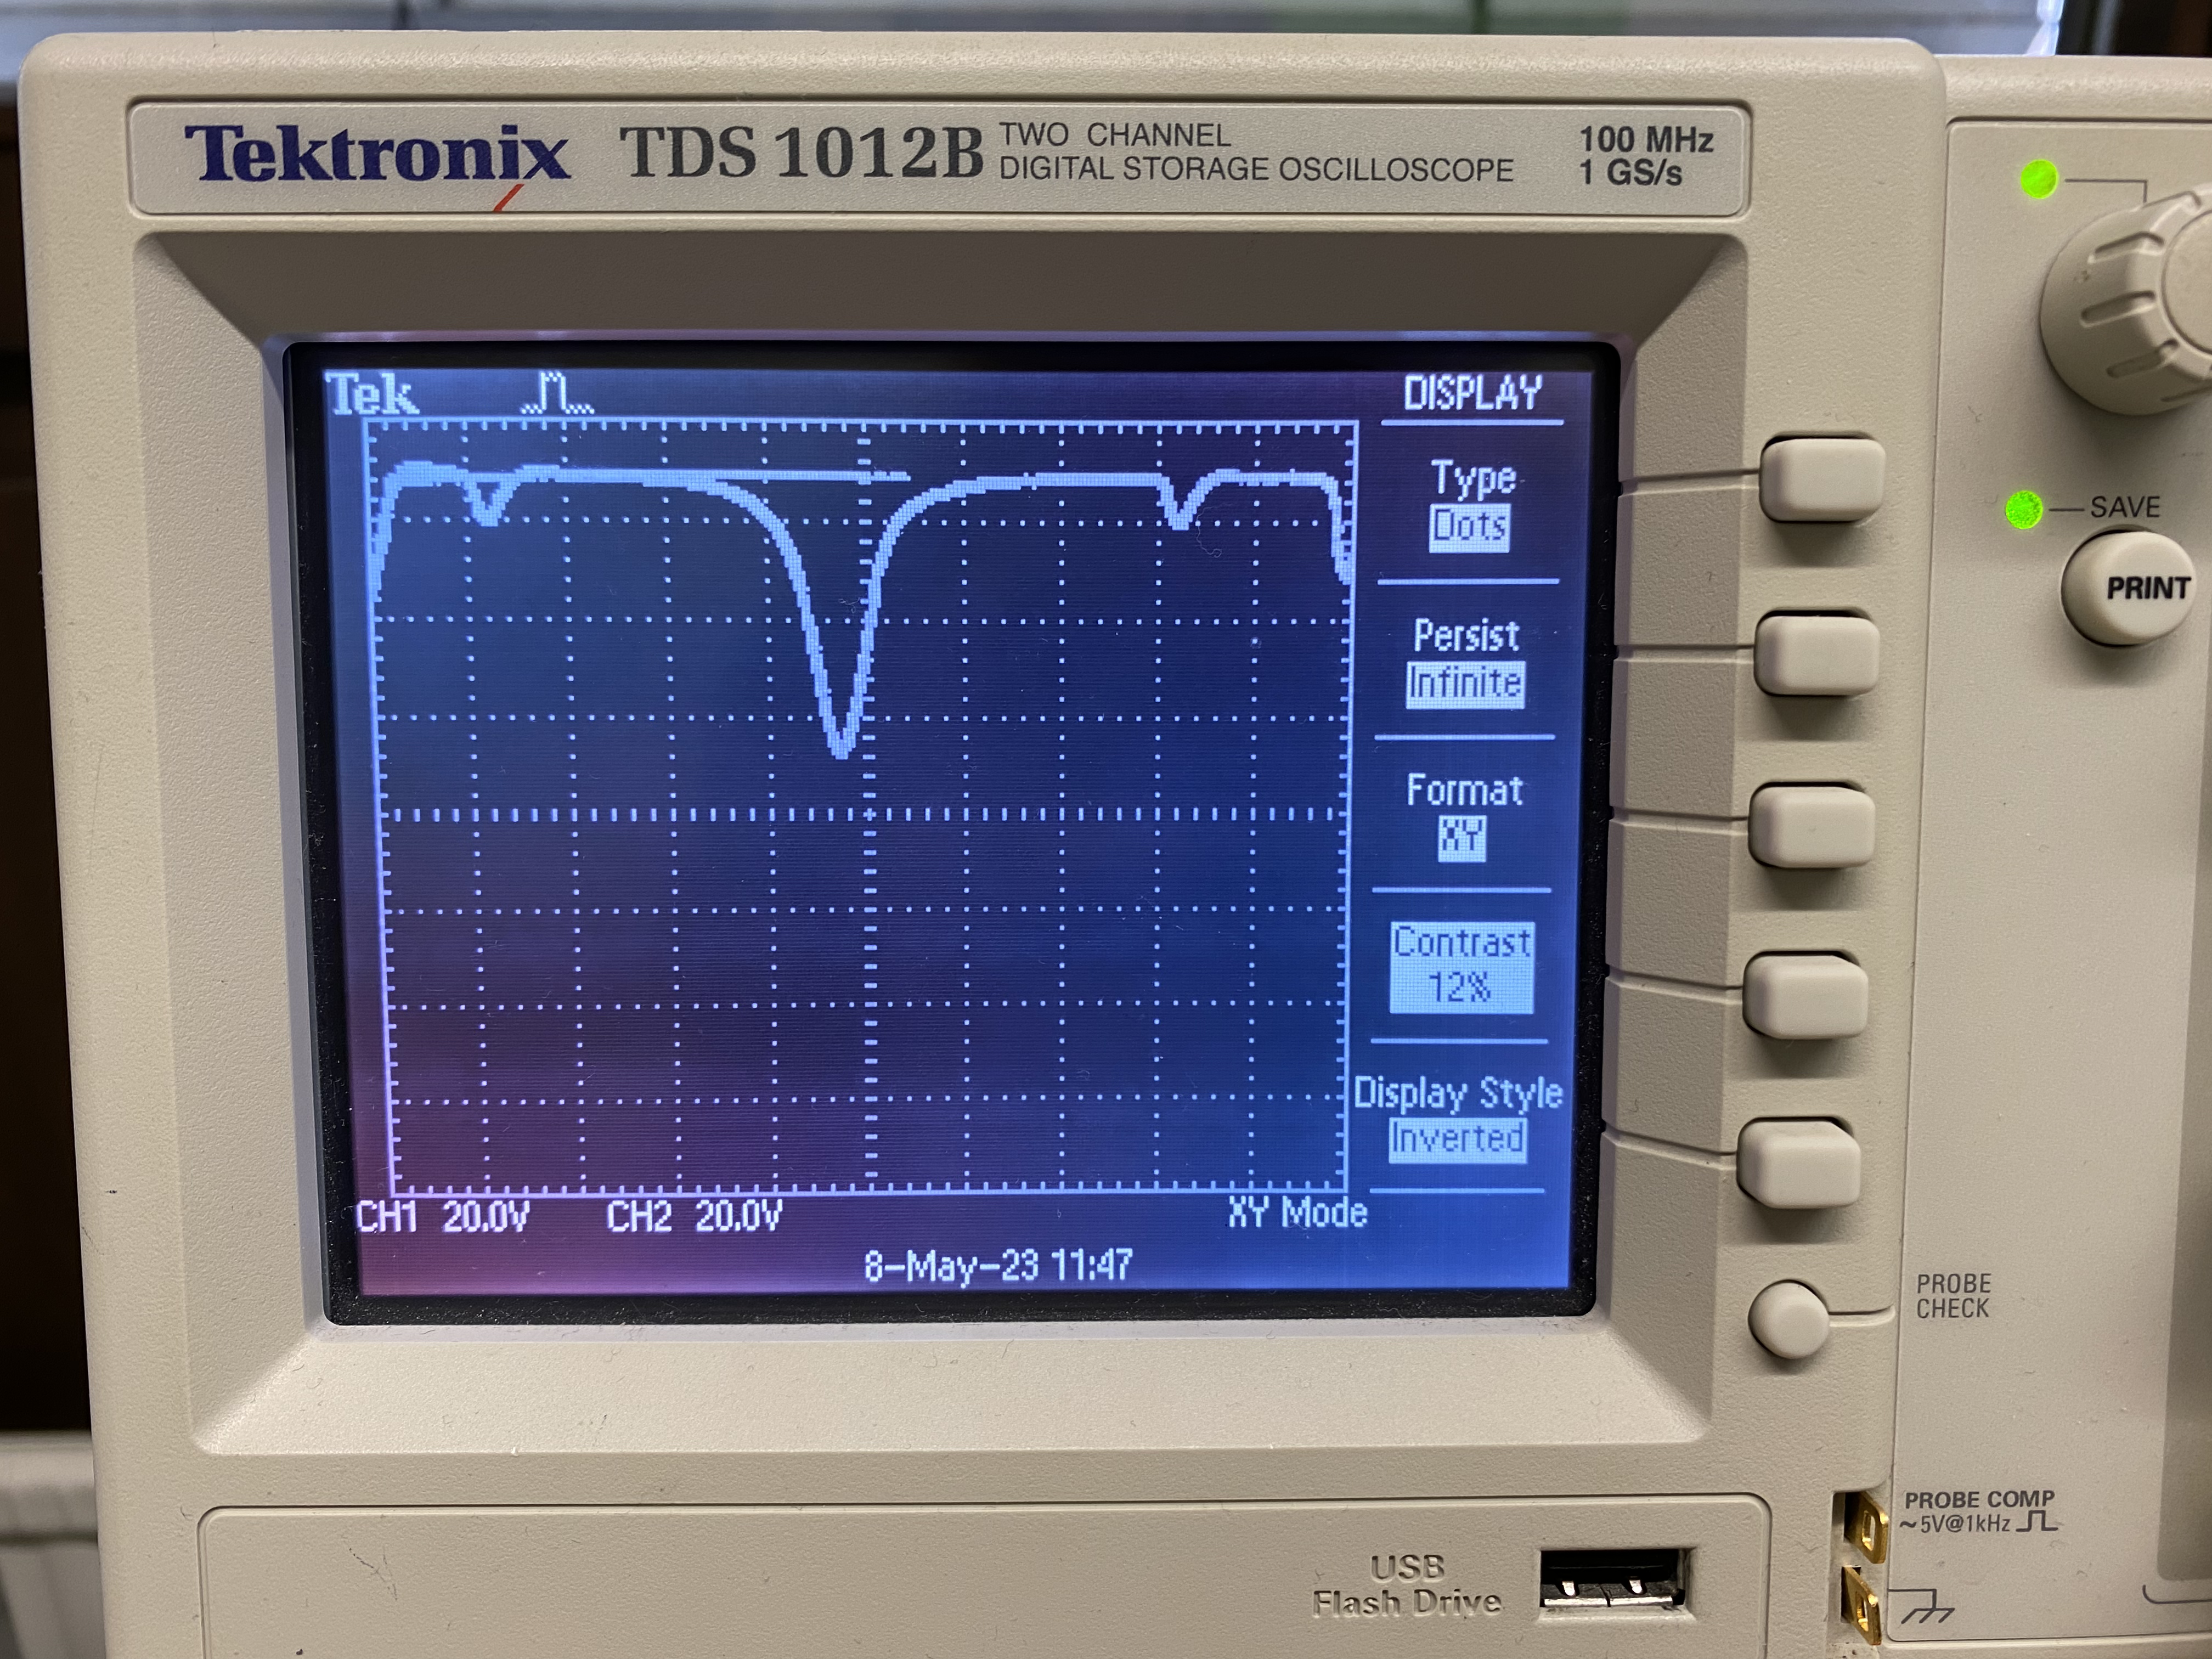
\includegraphics[width=0.7\textwidth]{data/Oszilloskop.png}
    \caption{Fotografie des Signalverlaufs bei $\SI{100}{\kilo\hertz}$.}
    \label{fig:Oszilloskop}
\end{figure}

Damit folgt das Amplitudenverhältnis zu
\begin{align*}
    A_1 &= 0.2, \\
    A_2 &= 0.5, \\
    \Rightarrow \frac{A_1}{A_2} &= 0.4.
\end{align*}
Es folgt demnach ein Isotopenverhältnis von $\SI{40}{\percent}$.

\subsection{Bestimmen des quadratischen Zeeman-Effektes}
\label{subsec:quadrZeeman}

Die Energiedifferenzen der Niveaus beim quadratischen Zeeman-Effekt werden mit der Gleichung (\ref{eq:quadratisch}) berechnet.
Mit den maximalen Magnetfeldern für die jeweiligen Resonanzstellen $B_1 = \SI{168.0873}{\micro\tesla}$ und $B_2 = \SI{230.4972}{\micro\tesla}$ folgt mit $m_F=2$ für $^{87}\text{Rb}$
und $m_F = 2$ für $^{85}\text{Rb}$ und der Hyperfeinstrukturaufspaltung, die sich aus Gleichung (\ref{eq:thermisch}) ergibt,
\begin{align*}
    W_1 &= \SI{4.93 \pm 0.05 e-09}{\eV}, \\
    W_2 &= \SI{4.60 \pm 0.08 e-09}{\eV}.
\end{align*}